\documentclass{article}
\usepackage[margin=1in]{geometry}
\usepackage{graphicx}
\usepackage{multicol}
\usepackage{cite}

\title{Project 2\\Tulsa Weather Prediction using a Feed-Forward Neural Network with a Sigmoid Activation Function and Supervised Learning Techniques}

\author{Christian Mann, Steven Reed}

\begin{document}

\maketitle

\begin{multicols}{2}

\begin{abstract}
In this paper we develop our own Feed-Forward Neural Network based off of previous examples found in the book and on the Internet. The Neural Network features Backpropogation for supervised learning. We then use it to approximate various functions. First we approximate the simple XOR function, then we attempt to approximate the behavior of weather in Tulsa, OK.
\end{abstract}

\section{Introduction}

A Neural Network is an abstract concept derived from studies in neuroscience. The general concept behind the structure of a Neural Network is simple to understand, yet it proves to be an incredibly difficult challenge to create a network of use. The purpose of a Neural Network is, in short, to approximate a function. Sometimes this function is known explicitly, but is difficult or expensive to compute. Other times the function cannot be explicitly known, but we can gather empirical data relating to the function. With a Neural Network, the goal is to approximate these functions using what information we have available about them.

There are two main techniques in developing the structure of a Neural Network. One technique is called Supervised Learning, in which the Network is ``trained'' by means of giving it example inputs and outputs from the function we want it to approximate. After pouring over the examples over and over, the Network (hopefully) becomes well equipped at evaluating those inputs, as well as similar ones. It does this by making many small changes to the weights associated with the edges in the network using a method known as ``backpropogation'' \cite{trappenberg}. The second popular method for constructing a Neural Network is known as Unsupervised Learning; we do not use any Unsupervised Learning techniques in this project.

In this project we wrote our own Neural Network in C++. We then used it to approximate various functions. These functions included the XOR function, a parametric circle, a parametric coffee cup, and ultimately using Tulsa weather data to predict Tulsa weather. The detailed parametric functions used were acquired via the Wolfram Alpha search engine \cite{wolfram}.

\section{Building a Neural Network}

We began by researching existing Neural Networks to get an idea for what kind of elements should be present in a network. There are many already availabe, and all have a varying set of features and capabilities. Many implementations are able to take advantage of a computer's GPU to parallelize the computations. The most simplistic example Network we could find, though, was a Javascript implementation known as Brain.js \cite{brain}. We used Brain.js as a guide for creating our own Neural Network in C++ with the hopes of performing faster than Javascript at a lower level, but not near the performance of a GPGPU solution.

We chose to use the Sigmoid function, $S(t)$, for its simplicity and convenient derivative. The convenient derivative is important as it will be computed a lot during training. Using a non-linear activation function also keeps our network from being limited to approximating linear functions \cite{hornik}. The derivative is used to modify error terms for each node which are eventually used to effect the change in weight to incoming edges. Since the derivate of the sigmoid function is highest for values around 0 (and S(0) = 0.5), multiplying the error by the derivative tends to favors error associated with outputs where $S(output)\approx0.5$, in turn causing them to adjust weights quicker.

	\[S(t) = \frac{1}{1+e^{-t}}\]
	\[\frac{d}{dt}S(t) = S(t) * (1-S(t))\]

In addition to the use of the Sigmoid function for node activation, and an accompanying bias used to alter the total value of each node when determining activation, we discovered the use of a momentum factor in Brain.js which we also incorporated in our own model. The momentum is intended to help the network avoid local minimums by increasing the change made to a given edge by some fraction of the change made to the edge on the previous iteration of backproppogation. It is intutive to think of this as momentum; an edge that is changed a lot once will only be changed by a lesser amount after the course of several successive smaller changes.

\section{Approximating the XOR Function}

Once the network was approaching completion, the first function we used to begin testing the network was the simple, yet popular, XOR function. After some debugging and fine tuning, we were able to build a network of 5 nodes (2 input, 1 output, 1 hidden layer with 2 nodes) which was trained to approximate XOR. The only training patterns given were the 4 boolean expressions in Table~\ref{tab:xortable}, but they each one was used to train the network roughly 4000 times to achieve adequate results with a sufficiently low error. The results of the inputs being fed through the resulting trained network can be seen in the right hand column of Table~\ref{tab:xortable}.

However, we were not satisfied to know that XOR performed appropriately for exactly the inputs we fed it repeatedly until we recieved low error. We were curious what the rest of the domain looked like after training. What did $(I_1=0.34, I_2=0.64)$ look like. To see what the rest of the graph looked like, we fed the trained network various $X$ and $Y$ inputs. We were suprised to see the graceful 3D surface shown in Figure~\ref{fig:xor1} and Figure~\ref{fig:xor2}.

\section{Approximating a Parametric Circle}

Once we had the XOR function working properly, we wanted to step up the difficulty. Next we wanted to approximated a parametric function with one input as the $t$ value and two outputs for the $x$ and $y$ values. We created roughly 30 data points approximating the parametric plot of a circle, and trained the network for many iterations longer than the XOR function. We then used a validation set of 100 datapoints around the circle to see how the network performed. The result can be seen in Figure~\ref{fig:circle} where the red circle is the actual validation set, and the blue circle is the one approximated by the network.

\section{Approximating a Parametric Coffee Cup}

As a more difficult challenge in parametric plot approximations, we used Wolfram Alpha to generate a parametric plot drawing of a coffee cup. The training data of the original plot can be seen in Figure~\ref{fig:coffee1}. Various neural network dimensions were used to try to approximate this coffee cup, but in the end it proved far too complex to do in a small amount of time. After training the neural network for 3 Million iterations, the graph in Figure~\ref{fig:coffee4} was achieved. The red outline is the training data while the blue outline is the output of the neural network. It's clear that the training had some effect, but did not converge as well as we had hoped.

\section{Weather Prediction}

\section{Conclusion and Future Work}

\bibliographystyle{abbrv}
\bibliography{citations}

\end{multicols}

\begin{table}[ht]
	\caption{XOR Truth Table}
	\label{tab:xortable}
	\begin{center}
		\begin{tabular}{cc|cc}
		\hline
		\hline
		\textbf{$In_1$} & \textbf{$In_2$} & \textbf{$Out$} & NeuralNet \\
		\hline
			$0.0$ & $0.0$ & $0.0$ & $0.0062$\\
			$0.0$ & $1.0$ & $1.0$ & $0.9934$\\
			$1.0$ & $0.0$ & $1.0$ & $0.9934$\\
			$1.0$ & $1.0$ & $0.0$ & $0.0086$\\
		\hline

		\hline
		\end{tabular}
	\end{center}
\end{table}

\begin{figure}[tb]
	\begin{center}
		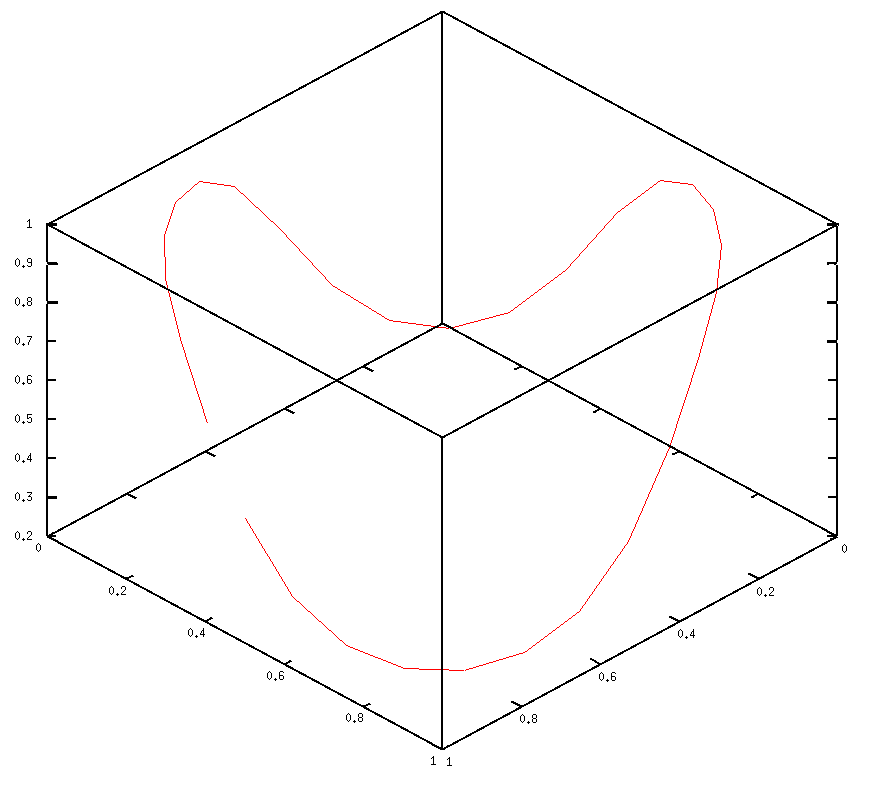
\includegraphics[scale=0.5]{img/xor1}
	\end{center}
	\caption{XOR function}
	\label{fig:xor1}
\end{figure}

\begin{figure}[tb]
	\begin{center}
		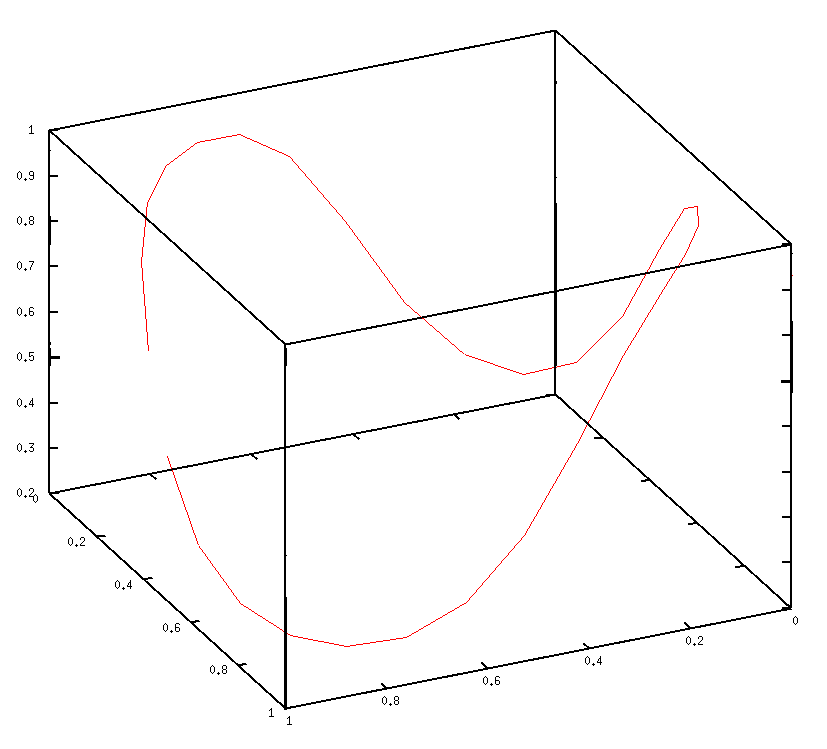
\includegraphics[scale=0.5]{img/xor2}
	\end{center}
	\caption{XOR Function}
	\label{fig:xor2}
\end{figure}

\begin{figure}[tb]
	\begin{center}
		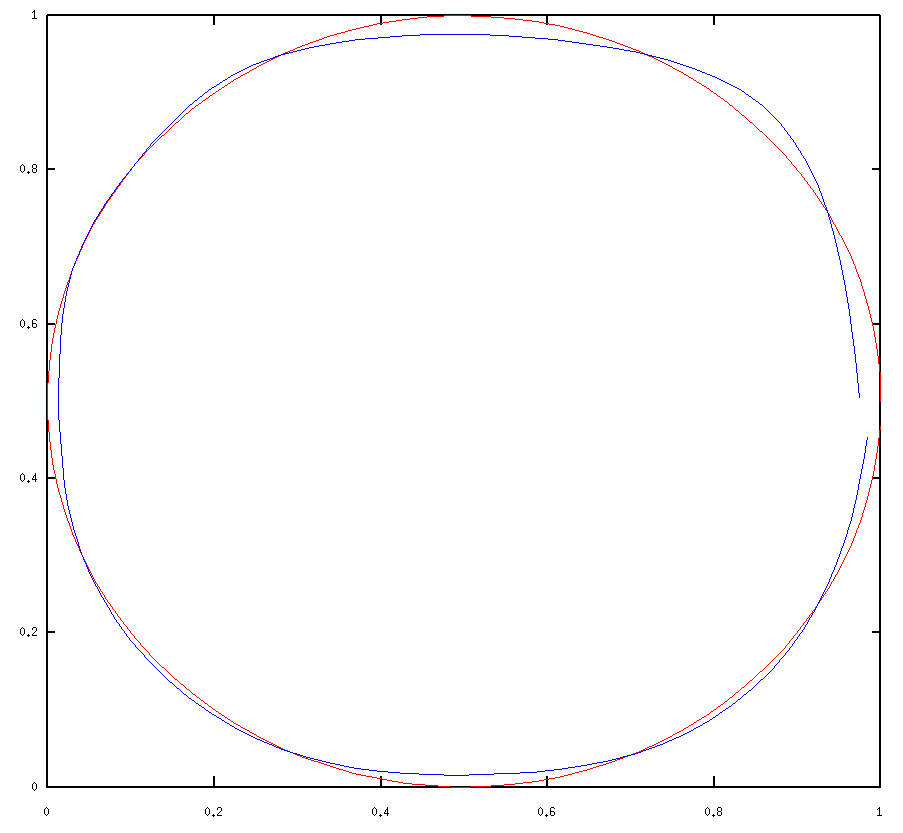
\includegraphics[scale=0.5]{img/circle}
	\end{center}
	\caption{Parametric Circle Function}
	\label{fig:circle}
\end{figure}

\begin{figure}[tb]
	\begin{center}
		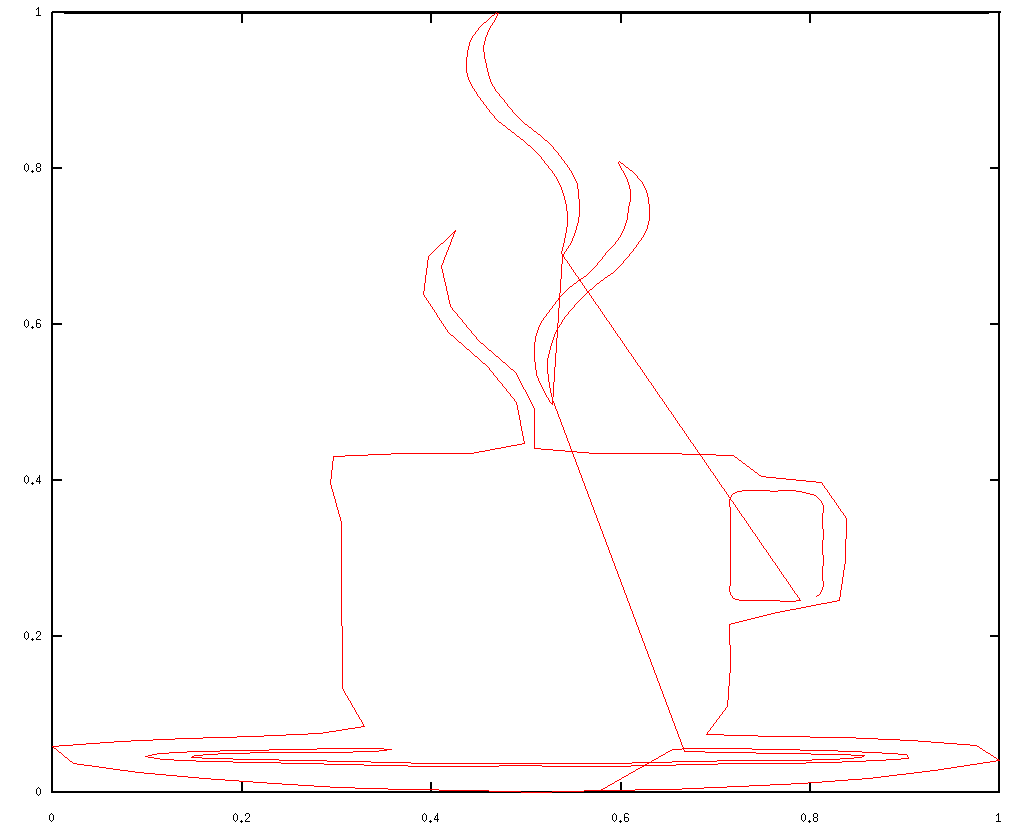
\includegraphics[scale=0.45]{img/coffee1}
	\end{center}
	\caption{Parametric Coffee Function}
	\label{fig:coffee1}
\end{figure}

\begin{figure}[tb]
	\begin{center}
		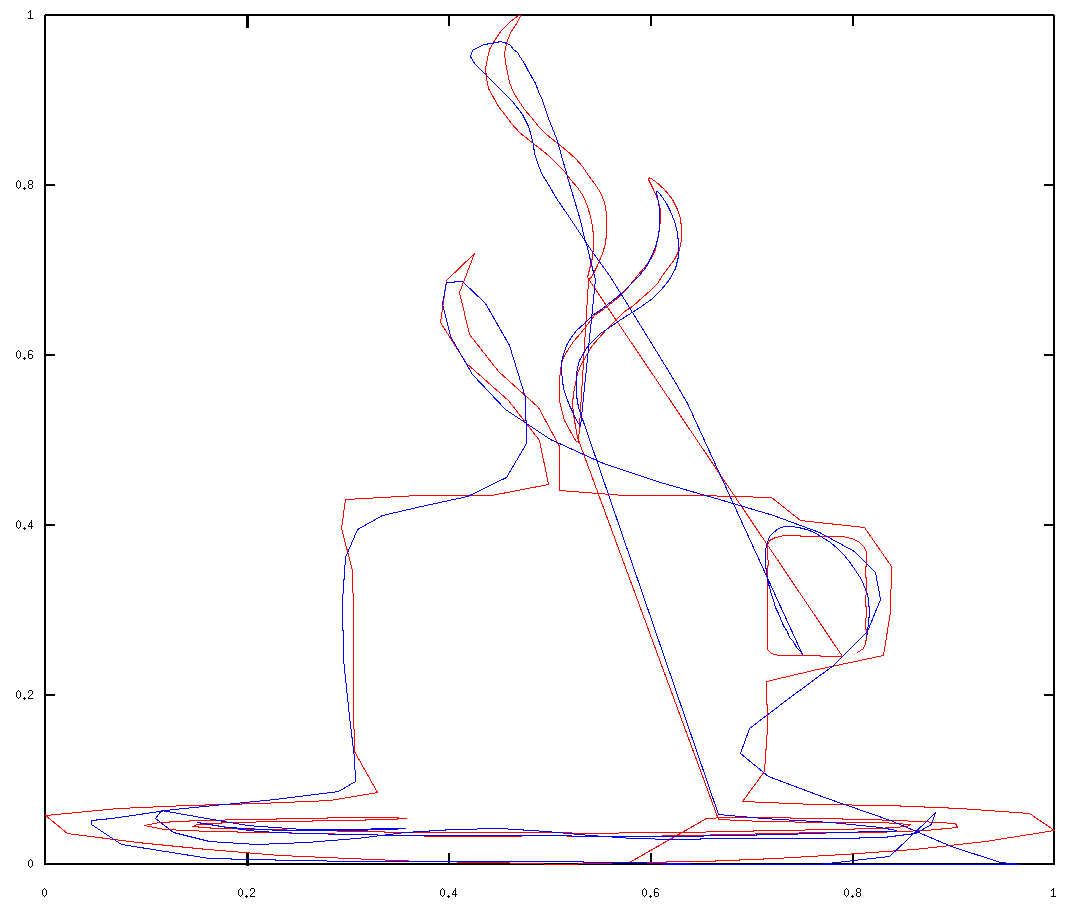
\includegraphics[scale=0.4]{img/coffee4}
	\end{center}
	\caption{Neural Coffee Approximation in Blue}
	\label{fig:coffee4}
\end{figure}

\end{document}

% citations:
% weather data